\documentclass[11pt,a4paper]{article}

\usepackage{amsmath,amssymb,amsfonts,amsthm}
\usepackage[ruled,vlined]{algorithm2e}
\usepackage{graphicx}
\usepackage{color}
\usepackage{hyperref}
\usepackage{cleveref}

% Commands for Inkscape figure
\newcommand{\St}{\mathcal{S}}

% Theorem environments
\newtheorem{theorem}{Theorem}
\newtheorem{definition}[theorem]{Definition}
\newtheorem{remark}[theorem]{Remark}

% Custom commands
\newcommand{\RV}[1]{\mathsf{#1}}           % Random variable
\newcommand{\PDF}[2][]{\Pr\left[#2\right]} % Probability
\newcommand{\Prob}[1]{\Pr\left[#1\right]}  % Probability
\newcommand{\fprate}{\varepsilon}          % False positive rate
\newcommand{\Card}[1]{\left|#1\right|}     % Cardinality
\newcommand{\Set}[1]{\mathcal{#1}}         % Set notation
\newcommand{\BitSet}{\{0,1\}}              % Bit set
\newcommand{\Null}{\mathsf{null}}
\newcommand{\False}{\mathsf{false}}
\newcommand{\Given}{\,|\,}
\newcommand{\hash}{\mathsf{H}}
\newcommand{\cat}{\,\|\,}                  % Concatenation

% Algorithm keywords
\SetKwFunction{MakeSingularHashSet}{make\_singular\_hash\_set}
\SetKwFunction{sampler}{random\_bit\_length}

\title{Singular Hash Sets: Random Bit Length Analysis}
\author{Alexander Towell}
\date{}

\begin{document}
\maketitle

\begin{abstract}
This note presents the probability mass function for the random bit length of Singular Hash Sets (SHS), a construction for oblivious set representation. We derive the distribution of the bit length required to achieve perfect collision for a given set cardinality and false positive rate, demonstrating that the PMF follows a telescoping sum structure that sums to unity.
\end{abstract}

\section{Introduction}

A \emph{Singular Hash Set} (SHS) is a compact representation of a set that achieves oblivious membership testing through cryptographic hash functions. The key insight is that we search for a random suffix $b_n$ such that all elements of the set hash to the same value when concatenated with this suffix.

The construction proceeds by testing increasingly longer bit strings until a ``perfect collision'' is found---where all set elements produce the same hash output. This note analyzes the probability distribution of the resulting bit length.

\section{Bit Length Sampling Algorithm}

\begin{algorithm}[H]
    \caption{Bit length sampler for Singular Hash Set}
    \label{alg:sampler}
    \SetKwProg{func}{function}{$\colon$}{}
    \KwIn{$m$ is the cardinality of the random set to approximate and $\fprate$ is the false positive rate.}
    \KwOut{A \emph{minimum bit length} $n$ of an SHS conditioned on a random set with cardinality $m$ and false positive rate $\fprate$.}
    \func{\sampler{$m$,$\fprate$}}{
        $\Set{S} \gets \emptyset$\;
        \For{$i \gets 1$ \KwTo $m$}{
            $x \gets $ randomly draw a bit string from $\BitSet^{*}$ without replacement\;
            $\Set{S} \gets \Set{S} \cup \{x\}$\;
        }
        $(h_k,b_n) \gets$ \MakeSingularHashSet{$\Set{S}$, $\fprate$}\;
        \Return $k + n + \mathcal{O}(1)$\;
    }
\end{algorithm}

For a particular $n$, each $b_n \in \BitSet^n$ may fail to result in a perfect collision, therefore $n$ is uncertain and takes on particular values with probabilities given by the following theorem.

\section{Random Bit Length Distribution}

\begin{definition}
\label{def:N_pmf}
The SHS generator finds a random string of a random bit length given by
\begin{equation}
    \RV{N} = \sampler(m, \fprate)\,,
\end{equation}
conditioned on a random set of cardinality $m$ and a false positive rate $\fprate$.
\end{definition}

\begin{theorem}[PMF of Random Bit Length]
\label{thm:N_pmf}
The random bit length $\RV{N}$ has a probability mass function given by
\begin{equation}
\label{eq:N_pmf}
    \PDF{[\RV{N} = n \Given m, \fprate]} = q^{2^n-1}\left(1 - q^{2^n}\right)\,,
\end{equation}
where $q = 1 - \fprate^{m-1}$, $m$ is the cardinality of the random set, and $\fprate$ is the false positive rate.
\end{theorem}

\begin{proof}
Consider that, approximately,
\begin{equation}
    \RV{N} = \log_2 \RV{Q}\,.
\end{equation}

Thus, the probability mass function is given by
\begin{align}
    \PDF{[\RV{N} = n \Given m,\fprate]}
        &= \Prob{\RV{N} = n}\\
        &= \Prob{\log_2 \RV{Q} = n}\\
        &= \Prob{\RV{Q} = 2^n}\\
        &= \PDF{[\RV{Q} = 2^n \Given m, \fprate]}\\
        &= \fprate^{m-1} (1 - \fprate^{m-1})^{2^n}
\end{align}

To verify this is a valid PMF, we must show that:
\begin{enumerate}
    \item Its image is a subset of $[0,1]$
    \item The summation over its domain equals $1$
\end{enumerate}

The first condition follows from the observation that $q$ is a positive number between $0$ and $1$, and therefore any non-negative power of $q$ is a positive number between $0$ and $1$.

The second condition is shown by calculating the infinite series:
\begin{align}
S &= \sum_{n=0}^{\infty} q^{2^n-1}\left(1-q^{2^n}\right)\\
&= \sum_{n=0}^{\infty} q^{2^n-1} - q^{2^{n+1}-1}\,.
\end{align}

Explicitly evaluating this series for the first few terms reveals a telescoping sum:
\begin{equation}
S = \underbrace{(1 - q)}_{n=0} + \underbrace{(q - q^3)}_{n=1} + \underbrace{(q^3 - q^7)}_{n=2} + \underbrace{(q^7 - q^{15})}_{n=3} + \cdots
\end{equation}

Everything cancels except $1$, confirming that $S = 1$.
\end{proof}

\section{Exact Oblivious Set Construction}

The following algorithm constructs an exact (zero false positive) oblivious set over a finite universal set.

\begin{algorithm}[H]
    \caption{Exact Singular Hash Set over a universal set $\Set{U}$}
    \label{alg:makeexactobset}
    \DontPrintSemicolon
    \SetKwProg{func}{function}{}{}
    \KwIn{$\Set{S}$ is a subset of a finite universal set $\Set{U}$. $k$ is any number in the set $\{1,2,\ldots\}$.}
    \KwOut{An \emph{oblivious} exact set of $\Set{S}$.}
    \func{\MakeSingularHashSet{$\Set{S}, k$}}{
        $\Set{S}_{\BitSet} \gets \left\{\mathsf{enc}_{\Set{U} \mapsto \BitSet}(x) \colon x \in \Set{S}\right\}$\;
        $\Set{\overline{S}}_{\BitSet} \gets \left\{\mathsf{enc}_{\Set{U} \mapsto \BitSet}(x) \colon x \in \Set{\overline{S}}\right\}$\;
        \tcp{Search for smallest bit string in ascending order}
        \For{$n \gets 0$ \KwTo $\infty$}{
            \For{$j \gets 1$ \KwTo $2^n$}{
                $\mathsf{found} \gets 1$\;
                \tcp{For maximum entropy, try bit strings randomly}
                $b_n \gets $ a bit string of length $n$ randomly drawn from $\BitSet^n$ without replacement\;
                $h_k \gets \Null$\;
                \For{$x \in \Set{S}_{\BitSet}$}{
                    \If{$h_k = \Null$}{
                        $h_k \gets \hash\!\left(x \cat b_n\right) \mod (k+1)$\;
                    }
                    \ElseIf{$h_k \neq \hash\!\left(x \cat b_n\right) \mod (k+1)$}{
                        $\mathsf{found} \gets \False$\;
                    }
                }
                \For{$x \in \Set{\overline{S}}_{\BitSet}$}{
                    \If{$h_k = \hash\!\left(x \cat b_n\right) \mod (k+1)$}{
                        $\mathsf{found} \gets \False$\;
                    }
                }
                \If{$\mathsf{found}$}{
                    \Return $(h_k, b_n)$\;
                }
            }
        }
    }
\end{algorithm}

\section{Space Complexity Analysis}

The exact oblivious set over a universe $\Set{U}$ has space complexity:
\begin{equation}
    k (\rho u - 1) + u \log_2(1 - 2^{-k})(\rho - 1)
\end{equation}
where $u = \Card{\Set{U}}$ and $\rho$ is the density of the set.

Per element in the universal set, the normalized complexity is:
\begin{equation}
    k\left(1 - \frac{1}{u \rho}\right) + \log_2\!\left(1 - 2^{-k}\right)\left(1 - \frac{1}{\rho}\right)
\end{equation}

For sets over the universe of bit strings up to length $n$, denoted by $\BitSet^{\leq n}$, there are $\Card{\BitSet^{\leq n}} = 2^{n+1} - 1$ bit strings. In this case, the set has a lower-bound space complexity of $\mathcal{O}(n)$.

\section{Space-Entropy Trade-off}

We may trade space complexity for entropy if desired. If the policy is to search for a bit string of length $t$ much larger than the expected bit length $-m \log_2 \fprate$, then:
\begin{equation}
    m < -\frac{t}{\log_2 \fprate}
\end{equation}

An estimator of the upper-bound on the cardinality is:
\begin{equation}
    \hat{m}_{\mathrm{max}} \approx -\frac{t}{\log_2 \fprate}
\end{equation}

The lower-bound is $0$ (the empty set), where the cardinality is uniformly distributed (maximum entropy) between $0$ and $\hat{m}_{\mathrm{max}}$, which has an entropy of:
\begin{equation}
    \log_2(1+\hat{m}_{\mathrm{max}})
\end{equation}

The \emph{absolute space efficiency} is now given by:
\begin{equation}
    \frac{m}{\hat{m}_{\mathrm{max}}}
\end{equation}
which is the maximum efficiency possible for an approximate set with cardinality uniformly distributed between $0$ and $\hat{m}_{\mathrm{max}}$.

\begin{remark}[Parameterized Efficiency]
Suppose $t = r \cdot m$ for some $r > 1$. Then:
\begin{equation}
    \hat{m}_{\mathrm{max}} \approx -\frac{r m}{\log_2 \fprate}
\end{equation}
which has an entropy of approximately:
\begin{equation}
    \log_2\!\left(1 -\frac{r m}{\log_2 \fprate}\right) \approx \log_2 r + \log_2 m + \log_2 \frac{1}{\fprate}
\end{equation}
and an absolute space efficiency of $1/r$.
\end{remark}

\section{Visualization}

Figure~\ref{fig:shs} illustrates the SHS construction. Elements $x_1, x_2, x_3$ from set $\Set{S}$ are concatenated with a suffix $y$ and hashed, with all elements mapping to the same hash bucket.

\begin{figure}[h]
\centering
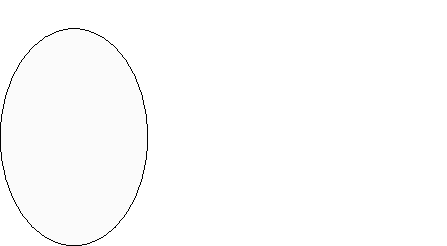
\includegraphics[width=0.7\columnwidth]{fig_shs.pdf}
\caption{Singular Hash Set construction. Set elements $\{x_1, x_2, x_3\}$ are each concatenated with suffix $y$ and hashed. When all hashes collide (map to the same value), the suffix $y$ becomes the oblivious representation of the set.}
\label{fig:shs}
\end{figure}

\section{Conclusion}

We have derived the probability mass function for the random bit length in Singular Hash Set constructions. The key result is that the PMF \eqref{eq:N_pmf} forms a telescoping series that sums to unity, providing a theoretical foundation for analyzing the expected storage requirements of SHS-based oblivious sets.

\end{document}
